%% abtex2-modelo-relatorio-tecnico.tex, v-1.7.1 laurocesar
%% Copyright 2012-2013 by abnTeX2 group at http://abntex2.googlecode.com/ 
%%
%% This work may be distributed and/or modified under the
%% conditions of the LaTeX Project Public License, either version 1.3
%% of this license or (at your option) any later version.
%% The latest version of this license is in
%%   http://www.latex-project.org/lppl.txt
%% and version 1.3 or later is part of all distributions of LaTeX
%% version 2005/12/01 or later.
%%
%% This work has the LPPL maintenance status `maintained'.
%% 
%% The Current Maintainer of this work is the abnTeX2 team, led
%% by Lauro César Araujo. Further information are available on 
%% http://abntex2.googlecode.com/
%%
%% This work consists of the files abntex2-modelo-relatorio-tecnico.tex,
%% abntex2-modelo-include-comandos and abntex2-modelo-references.bib
%%

% ------------------------------------------------------------------------
% ------------------------------------------------------------------------
% abnTeX2: Modelo de Relatório Técnico/Acadêmico em conformidade com 
% ABNT NBR 10719:2011 Informação e documentação - Relatório técnico e/ou
% científico - Apresentação
% ------------------------------------------------------------------------ 
% ------------------------------------------------------------------------

% Alterado por Rodrigo Campiolo para apresentação de relatórios na disciplina
% de Redes de Computadores II do Bacharelado em Ciência da Computação da UTFPR-CM.


\documentclass[
	% -- opções da classe memoir --
	12pt,				% tamanho da fonte
	%openright,			% capítulos começam em pág ímpar (insere página vazia caso preciso)
	oneside,   	        % para impressão em verso e anverso use twoside. Oposto a oneside
	a4paper,			% tamanho do papel. 
	% -- opções da classe abntex2 --
	%chapter=TITLE,		% títulos de capítulos convertidos em letras maiúsculas
	%section=TITLE,		% títulos de seções convertidos em letras maiúsculas
	%subsection=TITLE,	% títulos de subseções convertidos em letras maiúsculas
	%subsubsection=TITLE,% títulos de subsubseções convertidos em letras maiúsculas
	% -- opções do pacote babel --
	english,			% idioma adicional para hifenização
	french,				% idioma adicional para hifenização
	spanish,			% idioma adicional para hifenização
	brazil,				% o último idioma é o principal do documento
	]{pacotes/abntex2}


% ---
% PACOTES
% ---

% ---
% Pacotes fundamentais 
% ---
\usepackage{cmap}				% Mapear caracteres especiais no PDF
\usepackage{lmodern}			% Usa a fonte Latin Modern
\usepackage[T1]{fontenc}		% Selecao de codigos de fonte.
\usepackage[utf8]{inputenc}		% Codificacao do documento (conversão automática dos acentos)
\usepackage{indentfirst}		% Indenta o primeiro parágrafo de cada seção.
\usepackage{color}				% Controle das cores
\usepackage{graphicx}			% Inclusão de gráficos
% ---

% ---
% Pacotes adicionais, usados no anexo do modelo de folha de identificação
% ---
\usepackage{multicol}
\usepackage{multirow}
% ---
	
% ---
% Pacotes adicionais, usados apenas no âmbito do Modelo Canônico do abnteX2
% ---
\usepackage{lipsum}				% para geração de dummy text
% ---

% ---
% Pacotes de citações
% ---
\usepackage[brazilian,hyperpageref]{backref}	 % Paginas com as citações na bibl
\usepackage[alf]{pacotes/abntex2cite}	% Citações padrão ABNT
\usepackage{comment}

% ---
% Meus pacotes
% ---
\usepackage{float}
\usepackage{array}
% ---

% --- 
% CONFIGURAÇÕES DE PACOTES
% --- 

% ---
% Configurações do pacote backref
% Usado sem a opção hyperpageref de backref
\renewcommand{\backrefpagesname}{Citado na(s) página(s):~}
% Texto padrão antes do número das páginas
\renewcommand{\backref}{}
% Define os textos da citação
\renewcommand*{\backrefalt}[4]{
	\ifcase #1 %
		Nenhuma citação no texto.%
	\or
		Citado na página #2.%
	\else
		Citado #1 vezes nas páginas #2.%
	\fi}%
% ---

% ---
% Informações de dados para CAPA e FOLHA DE ROSTO
% ---
\titulo{Memória Virtual}
\autor{João Victor Briganti\\Luiz Gustavo Takeda}
\local{Campo Mourão}
\data{Novembro / 2024}
\instituicao{%
  Universidade Tecnológica Federal do Paraná -- UTFPR
  \par
  Departamento Acadêmico de Computação -- DACOM
  \par
  Bacharelado em Ciência da Computação -- BCC
}
\tipotrabalho{Relatório técnico}
% O preambulo deve conter o tipo do trabalho, o objetivo, 
% o nome da instituição e a área de concentração 
\preambulo{Relatório técnico de atividade prática solicitado pelo professor Rodrigo Campiolo na disciplina de Redes de Computadores II do Bacharelado em Ciência da Computação da Universidade Tecnológica Federal do Paraná.}
% ---

% ---
% Configurações de aparência do PDF final

% alterando o aspecto da cor azul
\definecolor{blue}{RGB}{41,5,195}

% informações do PDF
\makeatletter
\hypersetup{
     	%pagebackref=true,
		pdftitle={\@title}, 
		pdfauthor={\@author},
    	pdfsubject={\imprimirpreambulo},
	    pdfcreator={LaTeX with abnTeX2},
		pdfkeywords={abnt}{latex}{abntex}{abntex2}{relatório técnico}, 
		colorlinks=true,       		% false: boxed links; true: colored links
    	linkcolor=blue,          	% color of internal links
    	citecolor=blue,        		% color of links to bibliography
    	filecolor=magenta,      		% color of file links
		urlcolor=blue,
		bookmarksdepth=4
}
\makeatother
% --- 

% --- 
% Espaçamentos entre linhas e parágrafos 
% --- 

% O tamanho do parágrafo é dado por:
\setlength{\parindent}{1.3cm}

% Controle do espaçamento entre um parágrafo e outro:
\setlength{\parskip}{0.2cm}  % tente também \onelineskip

% ---
% compila o indice
% ---
\makeindex
% ---

% Omite a numeração de capítulos
\renewcommand*\thesection{\arabic{section}}



% ----
% Início do documento
% ----
\begin{document}

% Retira espaço extra obsoleto entre as frases.
\frenchspacing 

% ----------------------------------------------------------
% ELEMENTOS PRÉ-TEXTUAIS
% ----------------------------------------------------------
% \pretextual

% ---
% Capa
% ---
%\imprimircapa
% ---

% ---
% Folha de rosto
% (o * indica que haverá a ficha bibliográfica)
% ---
\imprimirfolhaderosto
% ---


% ---
% RESUMO
% ---

% resumo na língua vernácula (obrigatório)
\begin{resumo}
FAZER 
\vspace{\onelineskip}
    
 \noindent
 \textbf{Palavras-chave}: Processos; Escalonamento; Sistema Operacional.
\end{resumo}
% ---

% ---
% inserir lista de ilustrações
% ---
%\pdfbookmark[0]{\listfigurename}{lof}
%\listoffigures*
%\cleardoublepage
% ---

% ---
% inserir lista de tabelas
% ---
%\pdfbookmark[0]{\listtablename}{lot}
%\listoftables*
%\cleardoublepage
% ---

% ---
% inserir lista de abreviaturas e siglas
% ---
%\begin{siglas}
%  \item[IP] Internet Protocol
%  \item[TCP] Transmission Control Protocol
%  \item[UDP] User Datagram Protocol
%\end{siglas}
% ---

% ---
% inserir o sumario
% ---
\pdfbookmark[0]{\contentsname}{toc}
\tableofcontents*
\cleardoublepage
% ---

% ----------------------------------------------------------
% ELEMENTOS TEXTUAIS
% ----------------------------------------------------------
\textual

\makeatletter
\renewcommand{\chapter}{\@gobbletwo}
\makeatother

\section{Introdução}
\label{sec:introducao}

A virtualização de memória é um processo similar ao que o sistema operacional realiza com a virtualização da CPU, onde é criado a ilusão de que os processos estão sozinhos durante sua execução no hardware. Está virtualização é importante, ao proporcionar aos processos isolamento, proteção e, principalmente, a abstração de uma memória de modo que a mesma pareça infinita. Essa camada de abstração permite que os programadores não precisem se preocupar com o gerenciamento manual do posicionamento de variáveis e funções na memória física. Além disso, o sistema operacional pode otimizar o uso dos recursos de memória, possibilitando que múltiplos programas sejam carregados e executados simultaneamente, mesmo que a memória física disponível seja limitada~\cite{remzi2018}.

Um mecanismo utilizado para a implementação da memória virtual é a paginação. Neste mecanismo, a memória física é dividida em blocos de tamanho fixo, chamados de páginas, enquanto a memória virtual do processo é organizada em páginas virtuais de mesmo tamanho. O sistema operacional, com auxílio da MMU (\textit{Memory Management Unit}), mapeia as páginas virtuais para as páginas físicas, permitindo que um processo acesse sua memória de forma contígua e linear, mesmo que os dados estejam espalhados de forma não contígua na memória física. Além disso, a paginação facilita a alocação eficiente de memória, pois apenas as páginas realmente utilizadas precisam ser carregadas na RAM, enquanto as demais podem permanecer em dispositivos de armazenamento secundário, até que sejam necessárias. Essa técnica também contribui para o isolamento entre processos, já que cada um possui seu próprio espaço de endereçamento virtual, protegido de acessos indevidos por outros processos~\cite{tanenbaum2016}.

\section{Objetivos}
\label{sec:objetivos}
Os objetivos deste trabalho são compreender diferentes algoritmos para substituição de páginas da memória virtual, analisar os seus comportamentos com diferentes sobrecargas de trabalho e comparar o desempenho desses algoritmos.

\section{Fundamentação}
\label{sec:fundamentacao}
O gerenciamento da memória virtual é um processo que envolve a comunicação entre o sistema operacional e a MMU (\textit{Memory Management Unit}). Na paginação, a memória física é dividida em blocos de tamanho fixo, chamados de quadros, enquanto a memória virtual dos processos é organizada em blocos chamados de páginas. A MMU é responsável por traduzir os endereços virtuais das páginas para os quadros físicos correspondentes, que representam os endereços reais na memória RAM.

Como a MMU precisa traduzir todos os endereços acessados pelo processador, foi criada a TLB (\textit{Translation Lookaside Buffer}), uma cache que armazena as traduções de endereços mais frequentemente utilizadas. Quando um processo tenta acessar um endereço virtual, a MMU verifica primeiro se a tradução está presente na TLB. Caso esteja, a tradução é realizada rapidamente. Caso contrário, a MMU consulta a tabela de páginas na memória, resultando em um custo adicional de tempo.

Quando uma página solicitada por um processo não está presente na memória RAM, ocorre um \textit{page fault} (falha de página). Nesse caso, o sistema operacional decide qual página será substituída para trazer a nova página do disco para a RAM. Três algoritmos de substituição de páginas foram analisados neste trabalho~\cite{tanenbaum2016}:

\begin{itemize}
    \item FIFO (\textit{First In, First Out}): Substitui a página que está na memória há mais tempo, operando como uma fila onde a primeira página a entrar é a primeira a sair.
    \item LRU (\textit{Least Recently Used}): Substitui a página que não foi acessada há mais tempo, baseando-se no princípio de que páginas recentemente utilizadas têm maior probabilidade de serem acessadas novamente.
    \item NRU (\textit{Not Recently Used}): Uma variação do LRU que utiliza dois bits para classificar as páginas: o bit R (referência) e o bit M (modificação). A substituição segue a ordem de preferência:
    \begin{itemize}
        \item Páginas não referenciadas e não modificadas.
        \item Páginas não referenciadas e modificadas.
        \item Páginas referenciadas e não modificadas.
        \item Páginas referenciadas e modificadas.
    \end{itemize}
\end{itemize}

\section{Materiais}
\label{sec:materiais}

Simulador Amnesia~\cite{oliveira2008}.

\section{Procedimentos e Resultados}
\label{sec:procedimentos}
O simulador Amnesia foi utilizado para analisar métricas como tempos de execução e eficiência, avaliando o impacto de diferentes estratégias de substituição de páginas. Esse estudo permitiu observar o comportamento de cada algoritmo sob diversas cargas de trabalho, destacando como eles influenciam o desempenho e a eficiência do sistema.

Os testes foram conduzidos em arquiteturas que implementam os algoritmos de substituição de páginas, utilizando \textit{traces} de execução para simular e verificar o desempenho dessas arquiteturas em diferentes contextos.

Com exceção do algoritmo de paginação, todas as arquiteturas possuem a seguinte configuração:

\begin{itemize}
    \item CPU:
        \begin{itemize}
            \item \texttt{wordSize}: Tamanho da palavra da CPU, definido em 4 bytes.
        \end{itemize}
    
    \item Memória Principal:
        \begin{itemize}
            \item \texttt{blockSize}: Tamanho do bloco de memória, definido como 1 palavra (\textit{word}).

            \item \texttt{memorySize}: Tamanho total da memória principal, definido como 16 palavras (64 bytes).

            \item \texttt{cyclesPerAccessRead}: Número de ciclos necessários para realizar uma operação de leitura na memória principal, definido como 1 ciclo.

            \item \texttt{cyclesPerAccessWrite}: Número de ciclos necessários para realizar uma operação de escrita na memória principal, definido como 2 ciclo.
            
            \item \texttt{timeCicle}: Duração do tempo de cada ciclo, definido como 10 unidades de tempo.
        \end{itemize}
    
    \item Memória Virtual:
        \begin{itemize}
            \item \texttt{pageSize}: Tamanho da página de memória virtual, definido com 4 palavras (16 bytes).

            \item \texttt{diskMemorySize}: Tamanho total da memória em disco, definido como 16 páginas (256 bytes).

            \item \texttt{disckCiclesPerAccessRead}: Número de clicos necessários para ler uma página do disco, definido como 1 ciclo.

            \item \texttt{cyclesPerAccessWrite}: Número de ciclos necessários para escrever uma página no disco, definido como 2 ciclos.
            
            \item \texttt{timeCicle}: Duração de cada ciclo de disco, definido como 100 unidades de tempo.
        \end{itemize}
    
\end{itemize}

\subsection{Architecture-06-MM-16-VM(PS-4-DM-16-RA-FIFO)-TLB(none)}
\label{subsec:architecture-06}

Esta subseção descreve a Arquitetura-06, que utiliza o algoritmo FIFO para substituição de páginas na memória virtual.

Nesta arquitetura, o campo REP da tabela de páginas é utilizado para armazenar o tempo de entrada de cada página na memória. A página mais recentemente carregada recebe o valor máximo suportado pelo sistema, que no caso dos testes foi 3. Páginas que não estão presentes na memória são marcadas com o valor \texttt{0xFFFF}, indicando que estão ausentes. Quando ocorre um \textit{page fault}, o sistema seleciona para remoção a página cujo valor no campo REP seja 0. Após a remoção, os valores de REP de todas as páginas restantes são decrementados em 1, e a nova página, que anteriormente estava marcada com \texttt{0xFFFF}, é carregada na memória com o valor máximo. Esse mecanismo garante que a página mais antiga (com REP = 0) seja sempre substituída.

\subsubsection{TR\_5\_read\_and\_write\_20\_rand\_PS\_18}
\label{subsubsec:tr5-arch06}

A Figura~\ref{fig:tr5-arch06} mostra as informações sobre a execução do \textit{trace} TR\_5\_read\_and\_write\_20\_rand\_PS\_18 nesta arquitetura. O tempo total de execução deste \textit{trace} foi de 2210.
É possível observar que o maior tempo gasto desta arquitetura durante as execuções foi na memória principal, em especial nas operações de escrita, que tomaram um total de 74 ciclos e 740 unidades de tempo.

\begin{figure}[H]
  \centering
  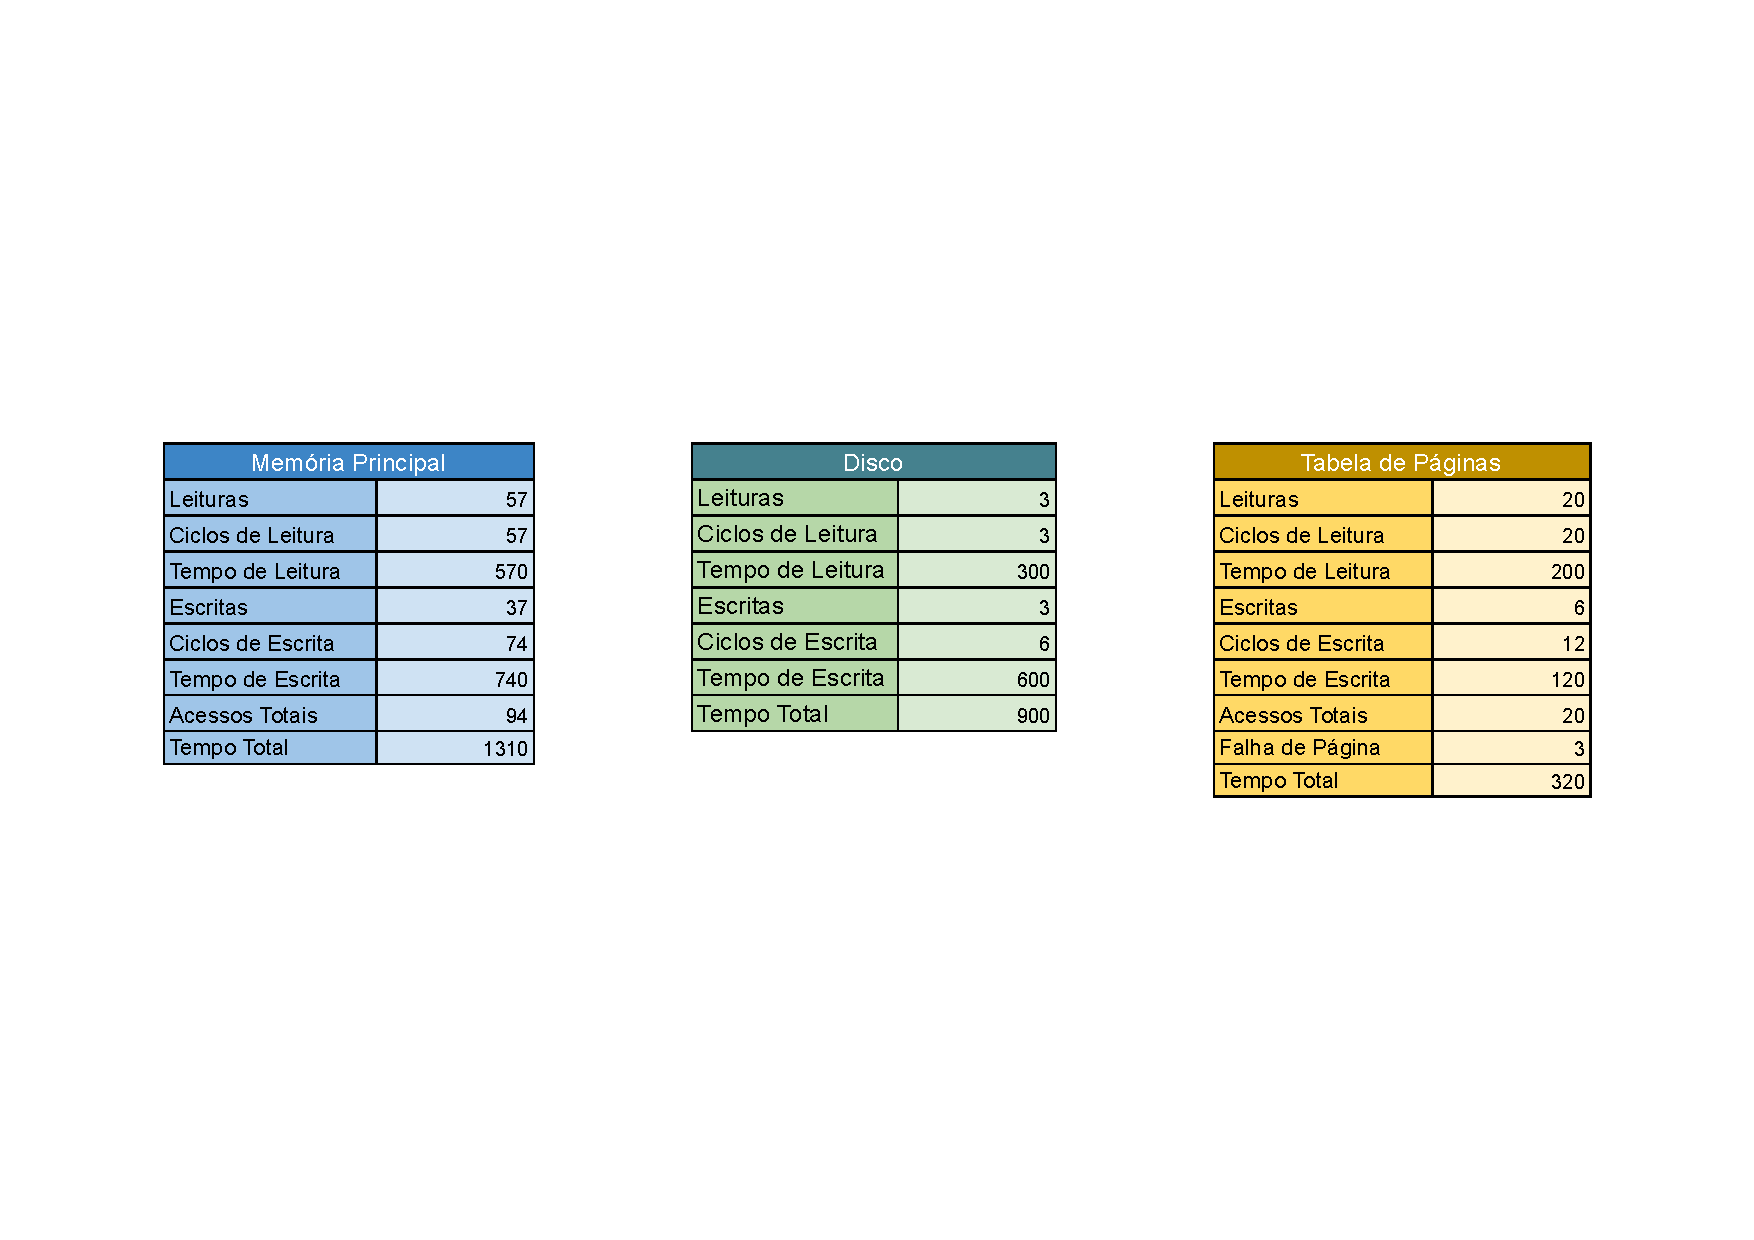
\includegraphics[scale=0.5]{figuras/Architecture06-TLB(none) TR5.pdf}
  \caption{Tabela com informações do \textit{trace} TR5 com a arquitetura que implementa o algoritmo FIFO.}
  \label{fig:tr5-arch06}
\end{figure}

\subsubsection{TR\_4\_read\_20\_cres\_PS\_20}
\label{subsubsec:tr4-arch06}

A Figura~\ref{fig:tr4-arch06} mostra as informações sobre a execução do \textit{trace} TR\_4\_read\_20\_cres\_PS\_20 nesta arquitetura. O tempo total de execução deste \textit{trace} foi de 980.
É possível observar que o maior tempo gasto desta arquitetura durante as execuções foi na memória principal, em especial nas operações de leitura, que tomaram um total de 48 ciclos e 480 unidades de tempo.

\begin{figure}[H]
  \centering
  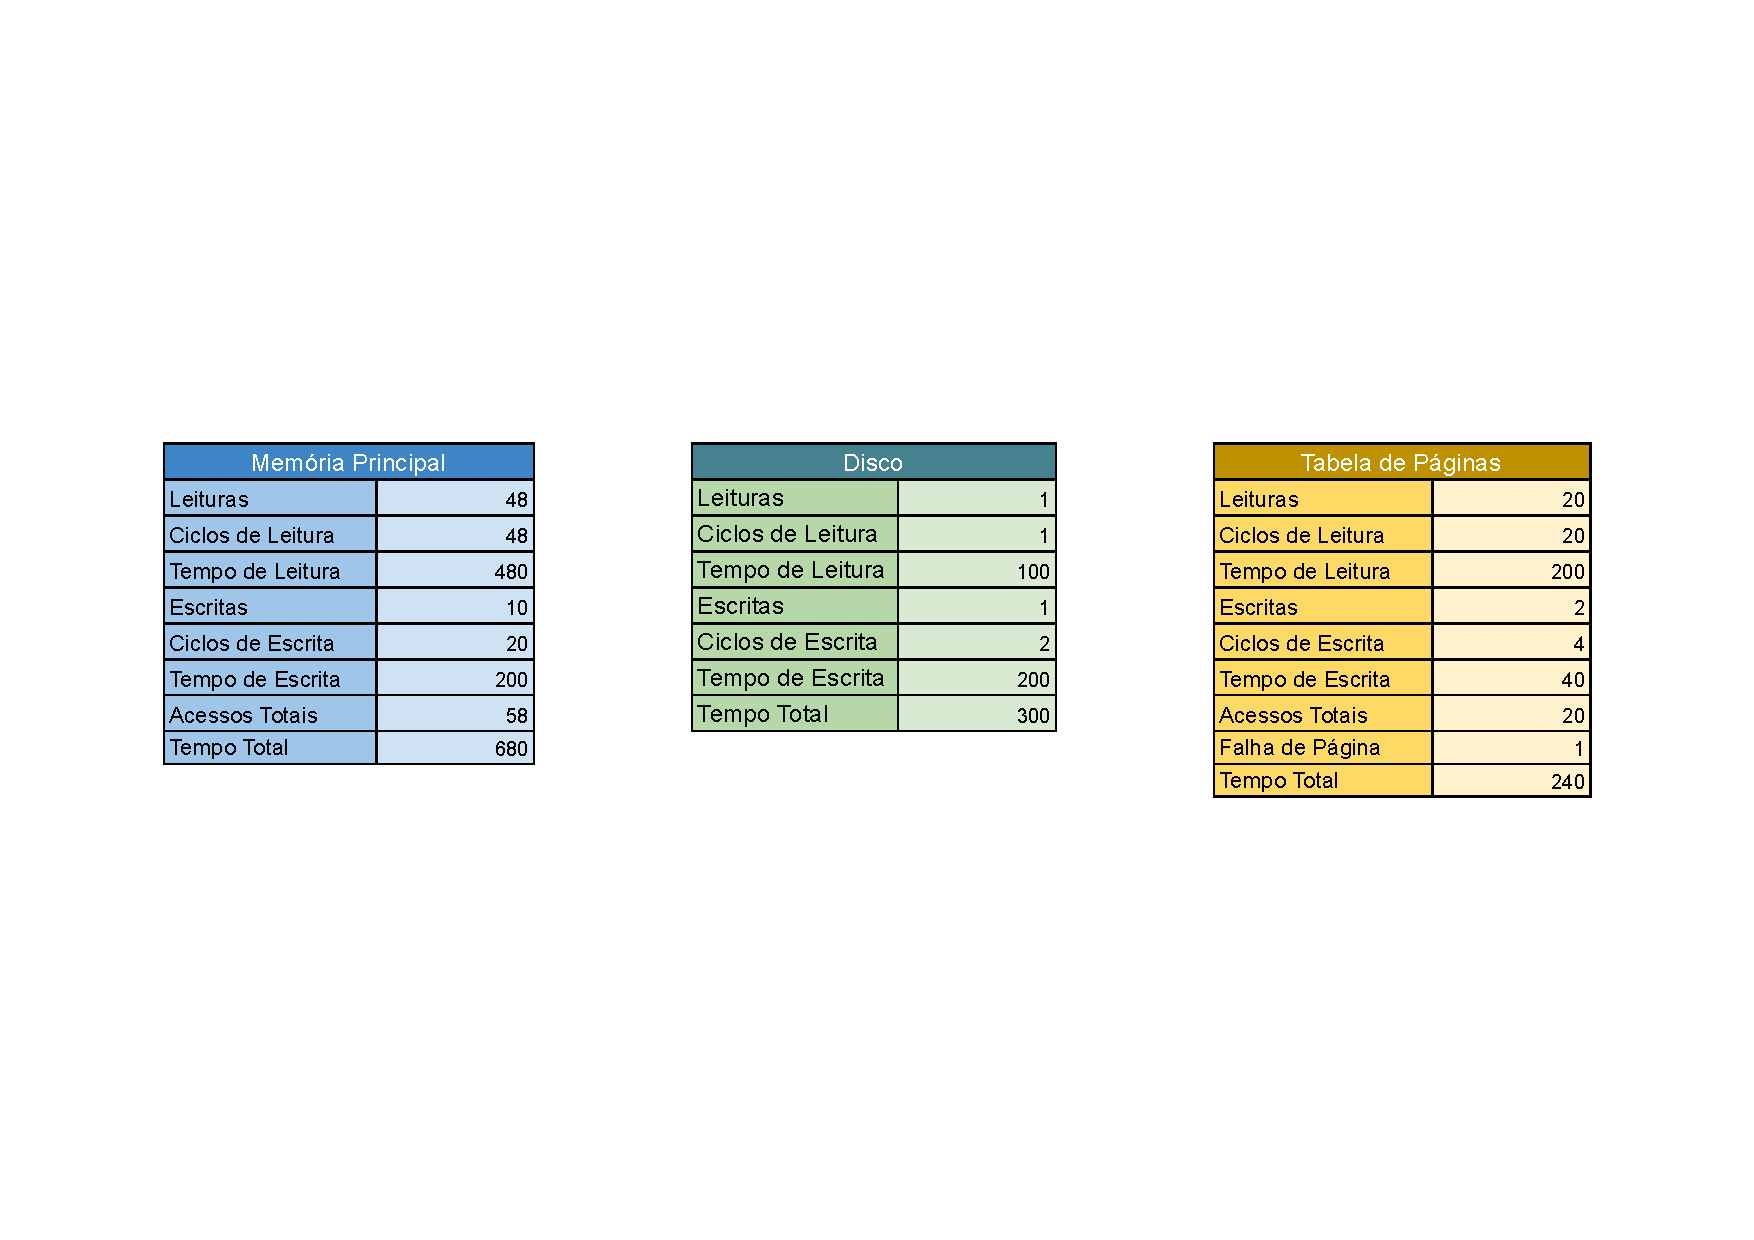
\includegraphics[scale=0.5]{figuras/Architecture06-TLB(none) TR4.pdf}
  \caption{Tabela com informações do \textit{trace} TR4 com a arquitetura que implementa o algoritmo FIFO.}
  \label{fig:tr4-arch06}
\end{figure}

\subsubsection{Comparação dos \textit{Traces}}
\label{subsubsec:comp-traces-arch6}

No primeiro \textit{trace}~\ref{subsubsec:tr5-arch06}, a arquitetura executa um programa que realiza operações de escrita e leitura em regiões aleatórias da memória. Já no segundo \textit{trace}~\ref{subsubsec:tr4-arch06}, o programa acessa as regiões de memória de forma sequencial e crescente. Essa diferença entre os dois \textit{traces} torna-se ainda mais evidente ao analisar os resultados gerados pelas execuções. É possível afirmar que o algoritmo FIFO apresenta um desempenho superior em situações onde o acesso à memória é sequencial, pois, nesses casos, as páginas mais antigas tendem a não ser reutilizadas, reduzindo a necessidade de substituições frequentes e, consequentemente, minimizando a ocorrência de \textit{page faults}.

\subsubsection{Análise das \textit{Page Faults}}
\label{subsubsec:analise-arch6}

\subsubsection{Uso da TLB}
\label{subsubsec:tlb-arch6}

\subsection{Architecture-07-MM-16-VM(PS-4-DM-16-RA-NRU)-TLB(none)}
\label{subsec:architecture-07}

Esta subseção descreve a Arquitetura-07, que utiliza o algoritmo NRU para substituição de páginas na memória virtual.

Nesta arquitetura, o campo REP da tabela de páginas é utilizado para armazenar o custo de remover está página da memória. O custo é calculado com base nos bits R e M, de leitura e modificação respectivamente, seu custo é calculado com base no seguinte:
\begin{itemize}
    \item \textbf{R = 0} e \textbf{M = 0}: Custo 0, páginas que não foram nem referenciadas, nem modificadas.

    \item \textbf{R = 0} e \textbf{M = 1}: Custo 1, páginas que só foram modificadas.

    \item \textbf{R = 1} e \textbf{M = 0}: Custo 2, páginas lidas recentemente.

    \item \textbf{R = 1} e \textbf{M = 1}: Custo 3, páginas que foram lidas e modificadas recentemente.
\end{itemize}

Páginas que não estão presentes na memória são marcadas com o valor \texttt{0xFFFF}, indicando que estão ausentes. Quando ocorre um \textit{page fault} o sistema escolhe a página com o menor custo, remove a mesma da memória, e carrega uma nova página na memória.

\subsubsection{TR\_6\_read\_and\_write\_30\_rand\_PS\_24}
\label{subsubsec:tr6-arch7}

A Figura~\ref{fig:tr6-arch07} mostra as informações sobre a execução do \textit{trace} TR\_6\_read\_and\_write\_30\_rand\_PS\_24 nesta arquitetura. O tempo total de execução deste \textit{trace} foi de 6450.
É possível observar que o maior tempo gasto desta arquitetura durante as execuções foi na memória principal, em especial nas operações de escrita, que tomaram um total de 210 ciclos e 2100 unidades de tempo.

\begin{figure}[H]
  \centering
  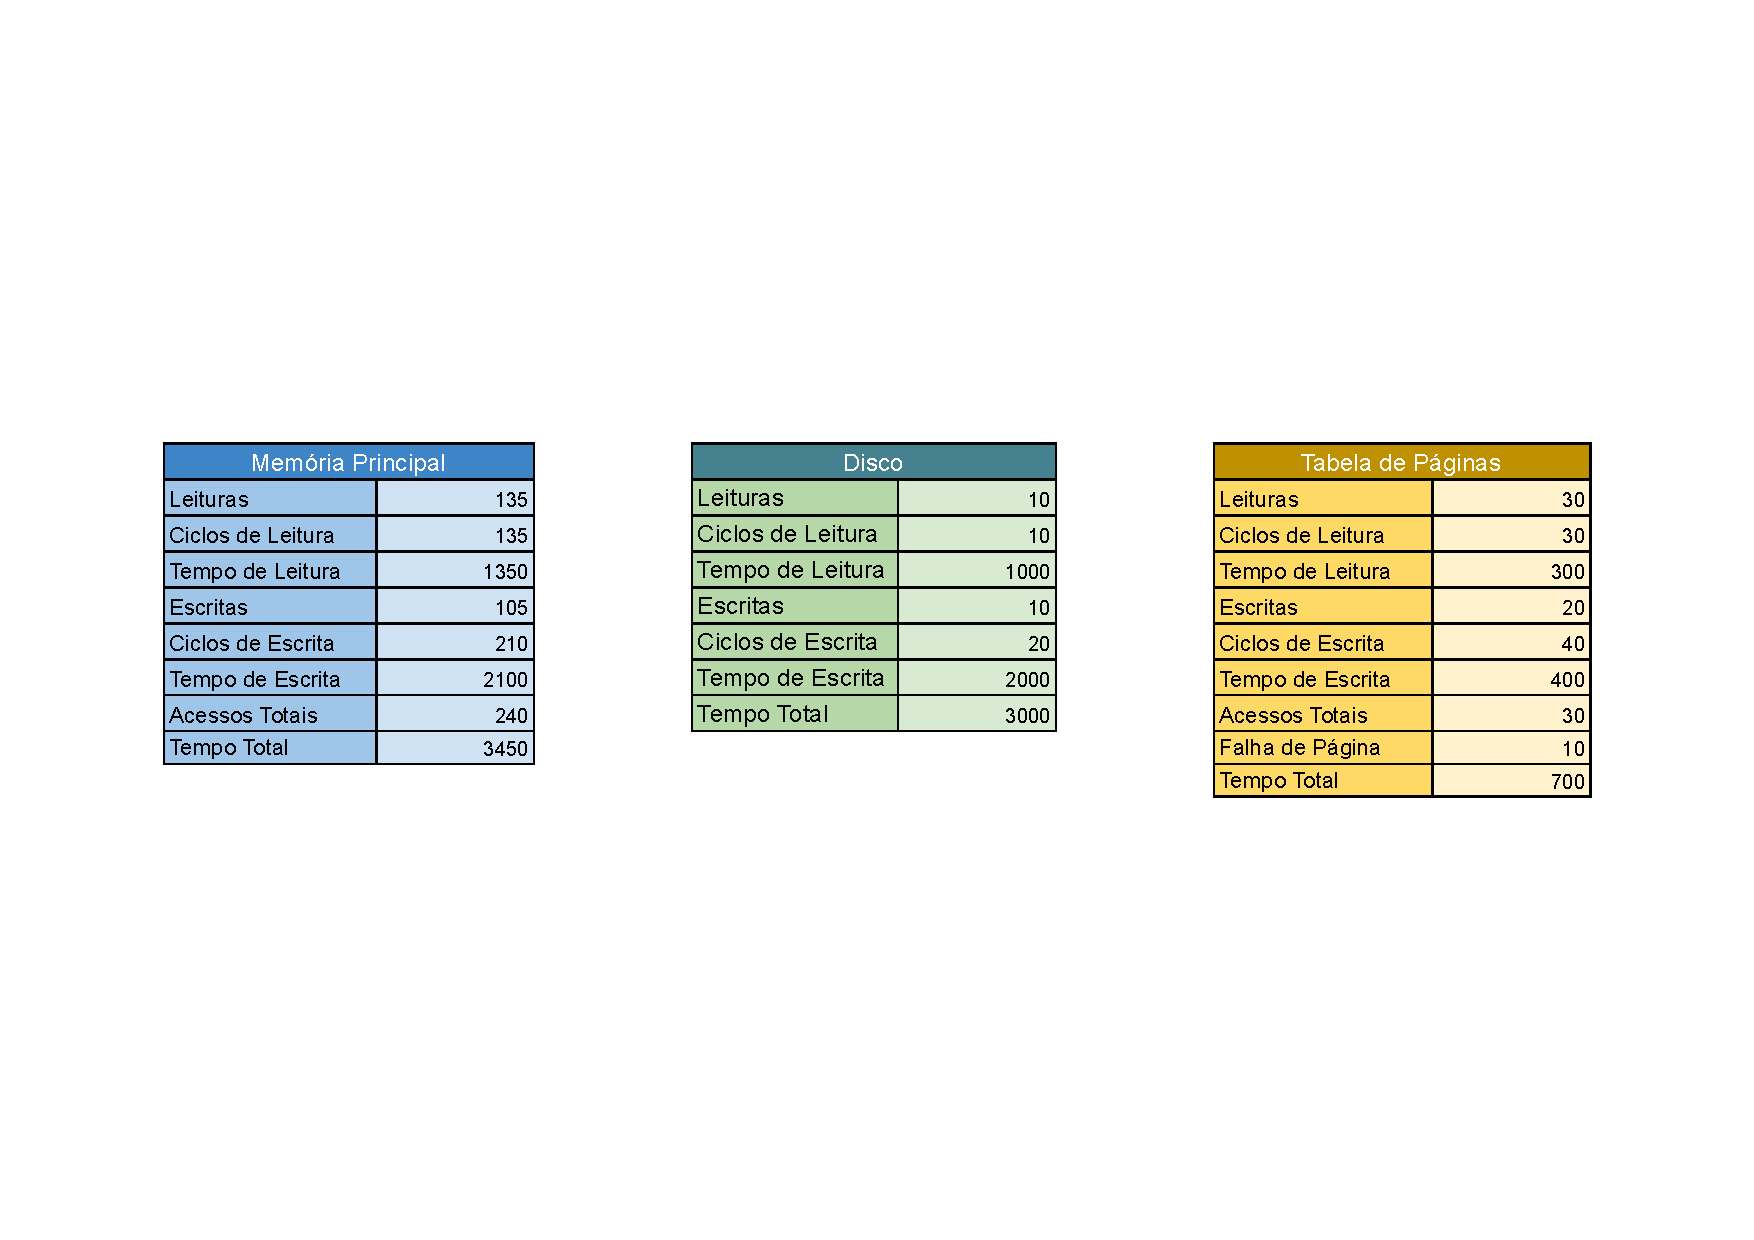
\includegraphics[scale=0.5]{figuras/Architecture07-TLB(none) TR6.pdf}
  \caption{Tabela com informações do \textit{trace} TR6 com a arquitetura que implementa o algoritmo NRU.}
  \label{fig:tr6-arch07}
\end{figure}

\subsubsection{TR\_5\_read\_and\_write\_20\_rand\_PS\_18}
\label{subsubsec:tr5-arch7}

A Figura~\ref{fig:tr5-arch07} mostra as informações sobre a execução do \textit{trace} TR\_5\_read\_and\_write\_20\_rand\_PS\_18 nesta arquitetura. O tempo total de execução deste \textit{trace} foi de 1050.
É possível observar que o maior tempo gasto desta arquitetura durante as execuções foi na memória principal, em especial nas operações de leitura, que tomaram um total de 41 ciclos e 410 unidades de tempo.

\begin{figure}[H]
  \centering
  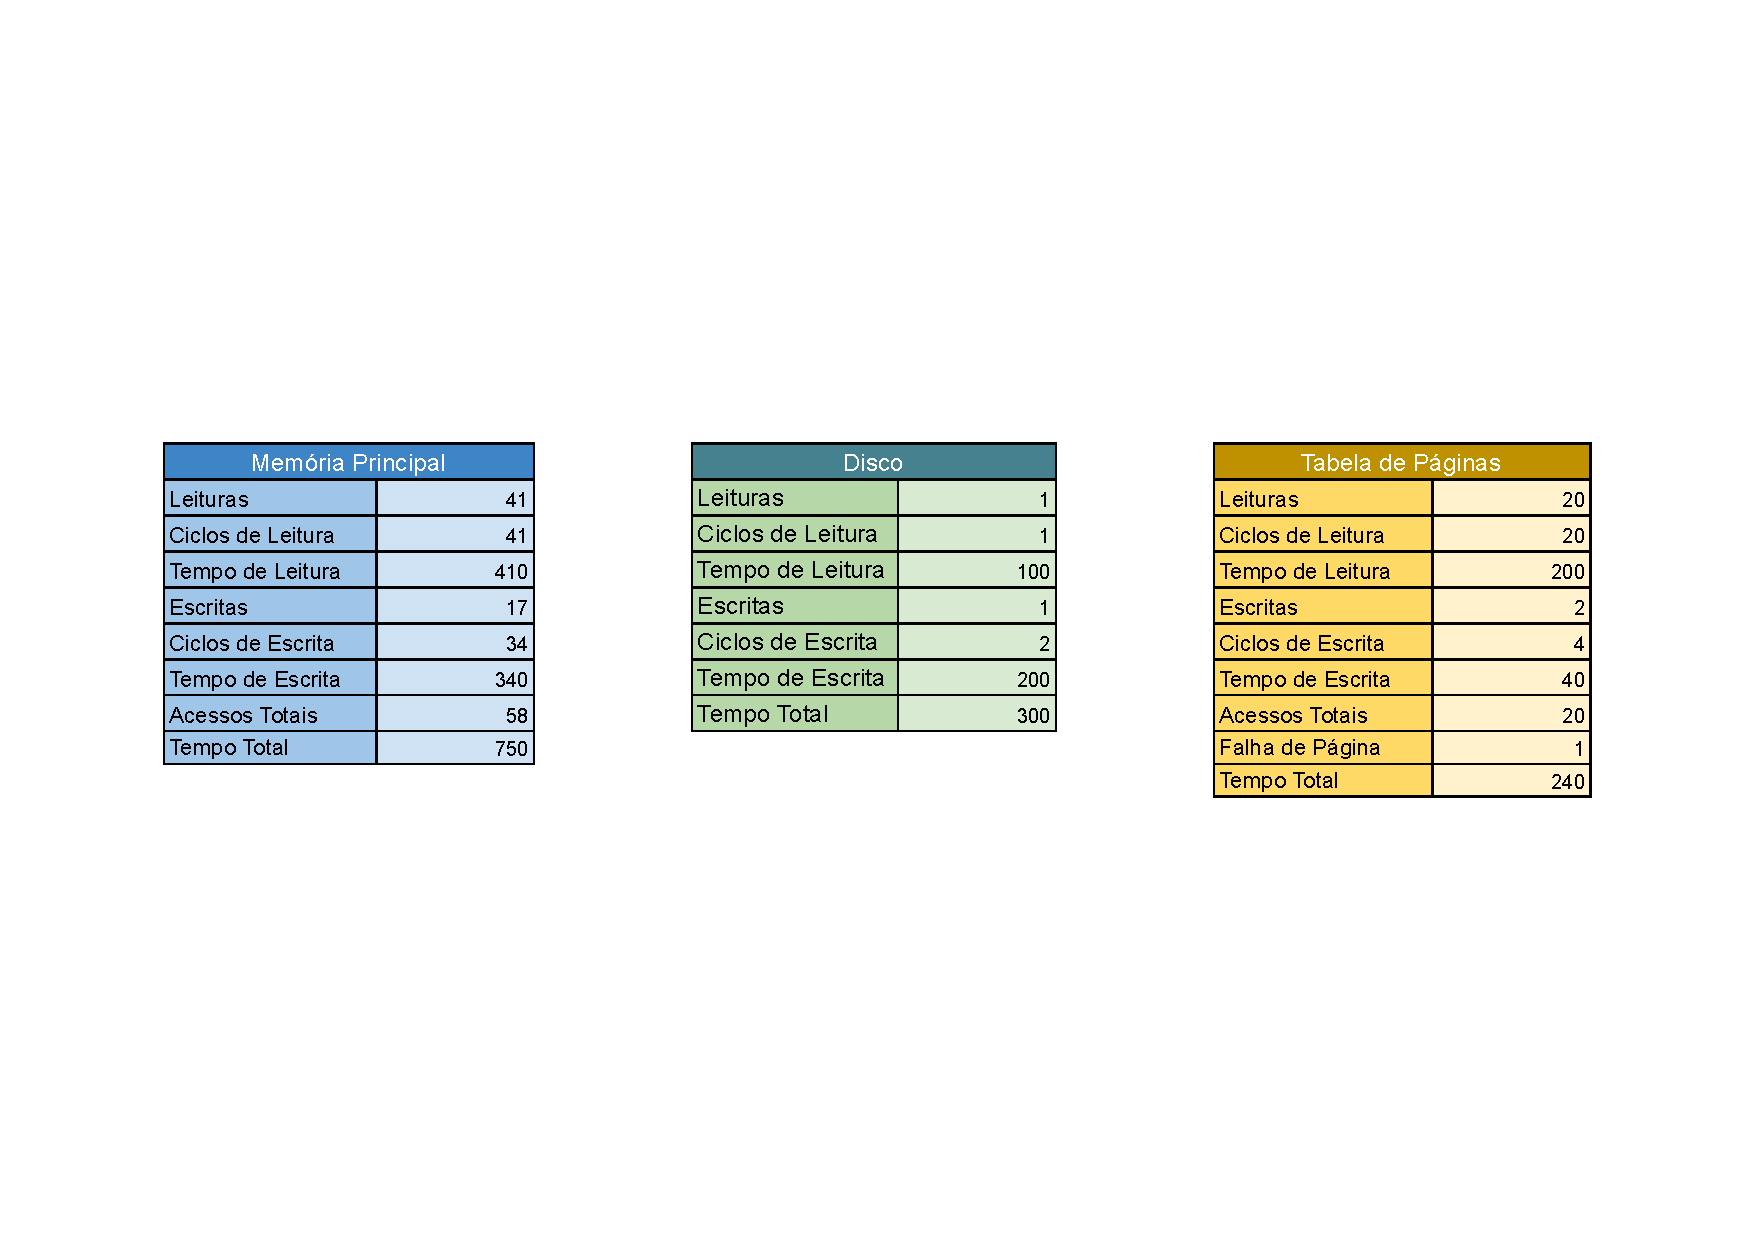
\includegraphics[scale=0.5]{figuras/Architecture07-TLB(none) TR5.pdf}
  \caption{Tabela com informações do \textit{trace} TR5 com a arquitetura que implementa o algoritmo NRU.}
  \label{fig:tr5-arch07}
\end{figure}

\subsubsection{Comparação dos \textit{Traces}}
\label{subsubsec:comp-traces-arch7}

Ambos os \textit{traces} envolvem programas que realizam operações de escrita e leitura em regiões aleatórias da memória. A principal diferença entre eles reside no fato de que o primeiro \textit{trace}~\ref{subsubsec:tr6-arch7} simula um \textit{loop}, o sugerindo um acesso à memória de maneira contígua a uma estrutura de dados, como um \textit{array}. Já o segundo \textit{trace}~\ref{subsubsec:tr5-arch7} parece representar uma função mais geral, com padrões de acesso menos previsíveis.

A partir desses cenários, é possível observar que o algoritmo NRU, embora apresente um desempenho superior ao FIFO em operações de acesso aleatório, não se mostra eficiente em contextos de acesso contíguo à memória. Durante a execução do primeiro \textit{trace}, ocorreu um fenômeno conhecido como \textit{thrashing}, onde páginas virtuais foram constantemente descartadas e recarregadas na memória. Esse comportamento impactou significativamente o tempo de execução, evidenciando uma das limitações do NRU neste cenário.

\subsubsection{Análise das \textit{Page Faults}}
\label{subsubsec:analise-arch7}

\subsubsection{Uso da TLB}
\label{subsubsec:tlb-arch7}

\subsection{Architecture-08-MM-16-VM(PS-4-DM-16-RA-LRU)-TLB(none)}
\label{subsec:architecture-08}

Esta subseção descreve a Arquitetura-08, que utiliza o algoritmo LRU para substituição de páginas na memória virtual.

Nesta arquitetura, o campo REP da tabela de páginas é utilizado para armazenar o momento em que uma página foi acessada pela última vez. Conforme as páginas são referenciadas, o valor do campo REP é incrementado, funcionando como um contador global que garante que cada novo acesso receba um valor maior que o anterior. Dessa forma, a página com o menor valor no campo REP é considerada a menos recentemente utilizada e, portanto, é selecionada para remoção quando ocorre um page fault. Novas páginas, ao serem carregadas na memória, recebem o maior valor disponível no contador REP, indicando que foram acessadas mais recentemente.

\subsubsection{TR\_6\_read\_and\_write\_30\_rand\_PS\_24}
\label{subsubsec:tr6-arch8}

A Figura~\ref{fig:tr6-arch08} mostra as informações sobre a execução do \textit{trace} TR\_6\_read\_and\_write\_30\_rand\_PS\_24 nesta arquitetura. O tempo total de execução deste \textit{trace} foi de 2390.
É possível observar que o maior tempo gasto desta arquitetura durante as execuções foi na memória principal, em especial nas operações de leitura, que tomaram um total de 79 ciclos e 790 unidades de tempo.

\begin{figure}[H]
  \centering
  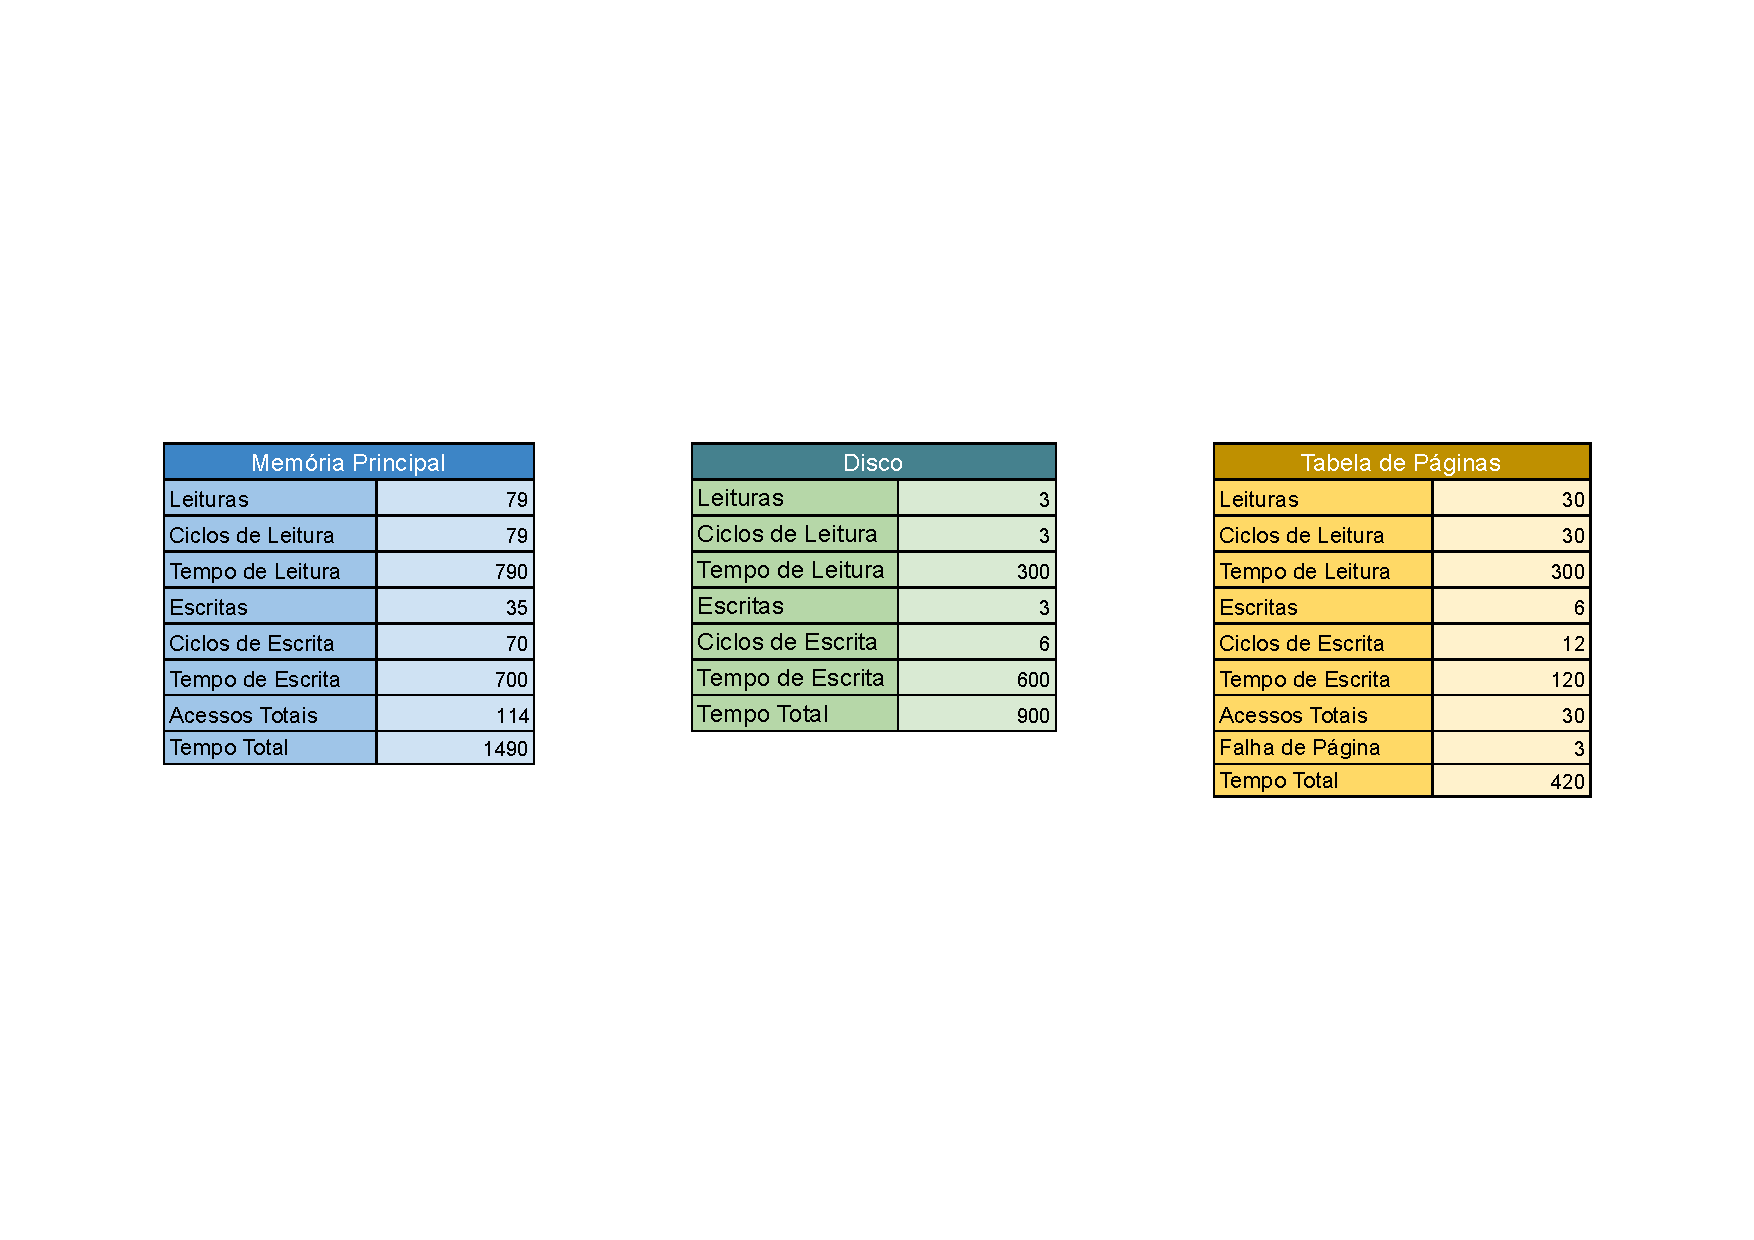
\includegraphics[scale=0.5]{figuras/Architecture08-TLB(none) TR6.pdf}
  \caption{Tabela com informações do \textit{trace} TR6 com a arquitetura que implementa o algoritmo LRU.}
  \label{fig:tr6-arch08}
\end{figure}

\subsubsection{Comparação dos \textit{Traces}}
\label{subsubsec:comp-traces-arch8}

Comparando o \textit{trace}~\ref{subsubsec:tr6-arch8}, executado por esta arquitetura com o algoritmo LRU, com o \textit{trace}~\ref{subsubsec:tr6-arch7}, executado pela arquitetura~\ref{subsec:architecture-07} com o algoritmo NRU, observa-se que o LRU apresenta uma vantagem significativa em termos de tempo de execução. O LRU conseguiu concluir o \textit{trace} em cerca de 3 vezes menos tempo que o NRU. 

Além disso, o LRU não sofreu com o fenômeno de \textit{thrashing}, que afetou severamente o desempenho do NRU. Enquanto o NRU utiliza uma abordagem aproximada, baseada nos bits de referência (R) e modificação (M), o LRU consegue identificar com precisão as páginas menos recentemente utilizadas, evitando substituições desnecessárias e consequentemente garantindo um uso mais eficiente da memória.

\subsubsection{Análise das \textit{Page Faults}}
\label{subsubsec:analise-arch8}

\subsubsection{Uso da TLB}
\label{subsubsec:tlb-arch8}

\subsection{Simulação dos Algoritmos}
\label{subsec:simulate}

Nesta seção todas as arquiteturas foram testadas com o mesmo \textit{trace}, que simula um pequeno \textit{loop} sendo executado.

\subsubsection{NRU}
\label{subsubsec:nru}

A Figura~\ref{fig:nru} mostra as informações sobre a execução do \textit{trace} na arquitetura utilizando o NRU. O tempo total de execução deste \textit{trace} foi de 2190.
É possível observar que o maior tempo gasto desta arquitetura durante as execuções foi na memória principal, em especial nas operações de escrita, que tomaram um total de 70 ciclos e 700 unidades de tempo.

\begin{figure}[H]
  \centering
  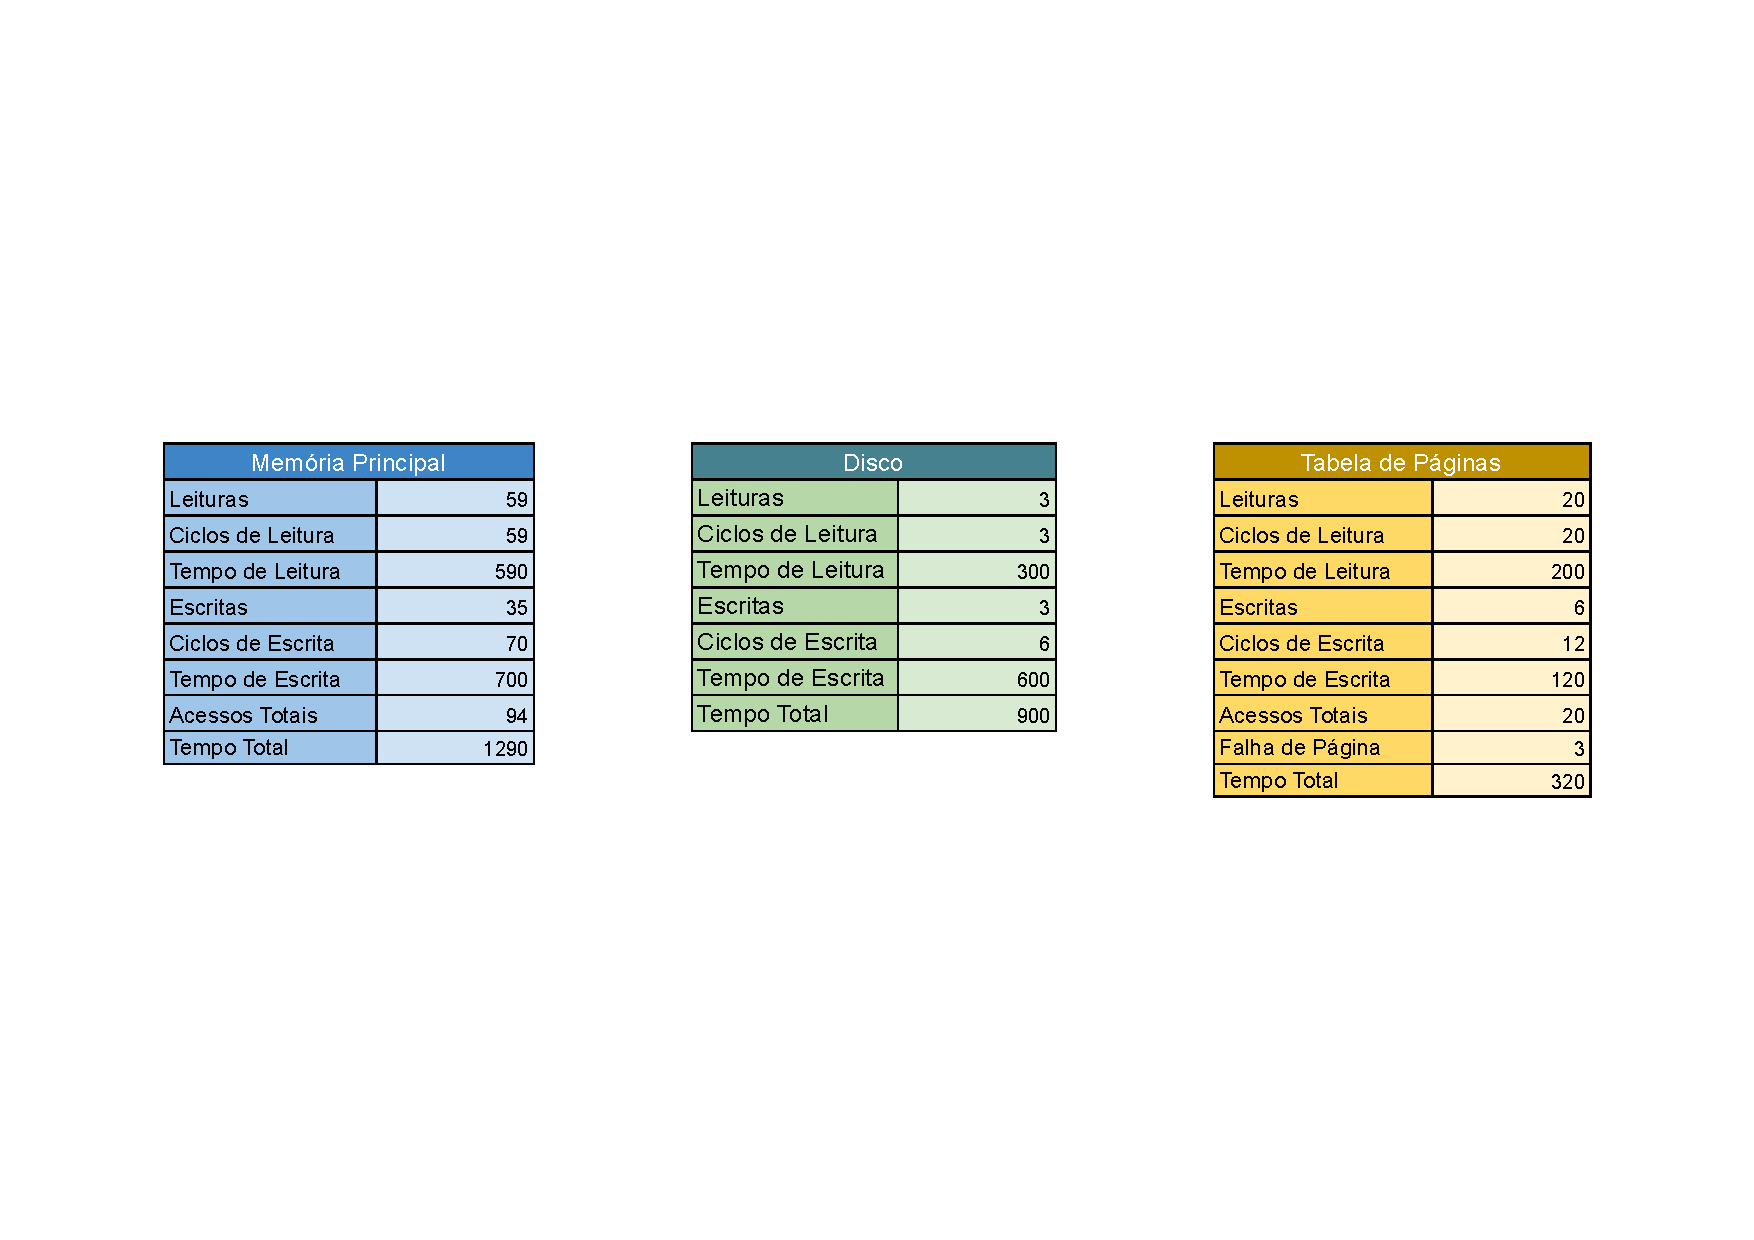
\includegraphics[scale=0.5]{figuras/NRU-TLB(none).pdf}
  \caption{Tabela com informações da execução do algoritmo NRU.}
  \label{fig:nru}
\end{figure}

\subsubsection{FIFO}
\label{subsubsec:fifo}

A Figura~\ref{fig:fifo} mostra as informações sobre a execução do \textit{trace} na arquitetura utilizando o FIFO. O tempo total de execução deste \textit{trace} foi de 2770.
É possível observar que o maior tempo gasto desta arquitetura durante as execuções foi na memória principal, em especial nas operações de escrita, que tomaram um total de 90 ciclos e 900 unidades de tempo.

\begin{figure}[H]
  \centering
  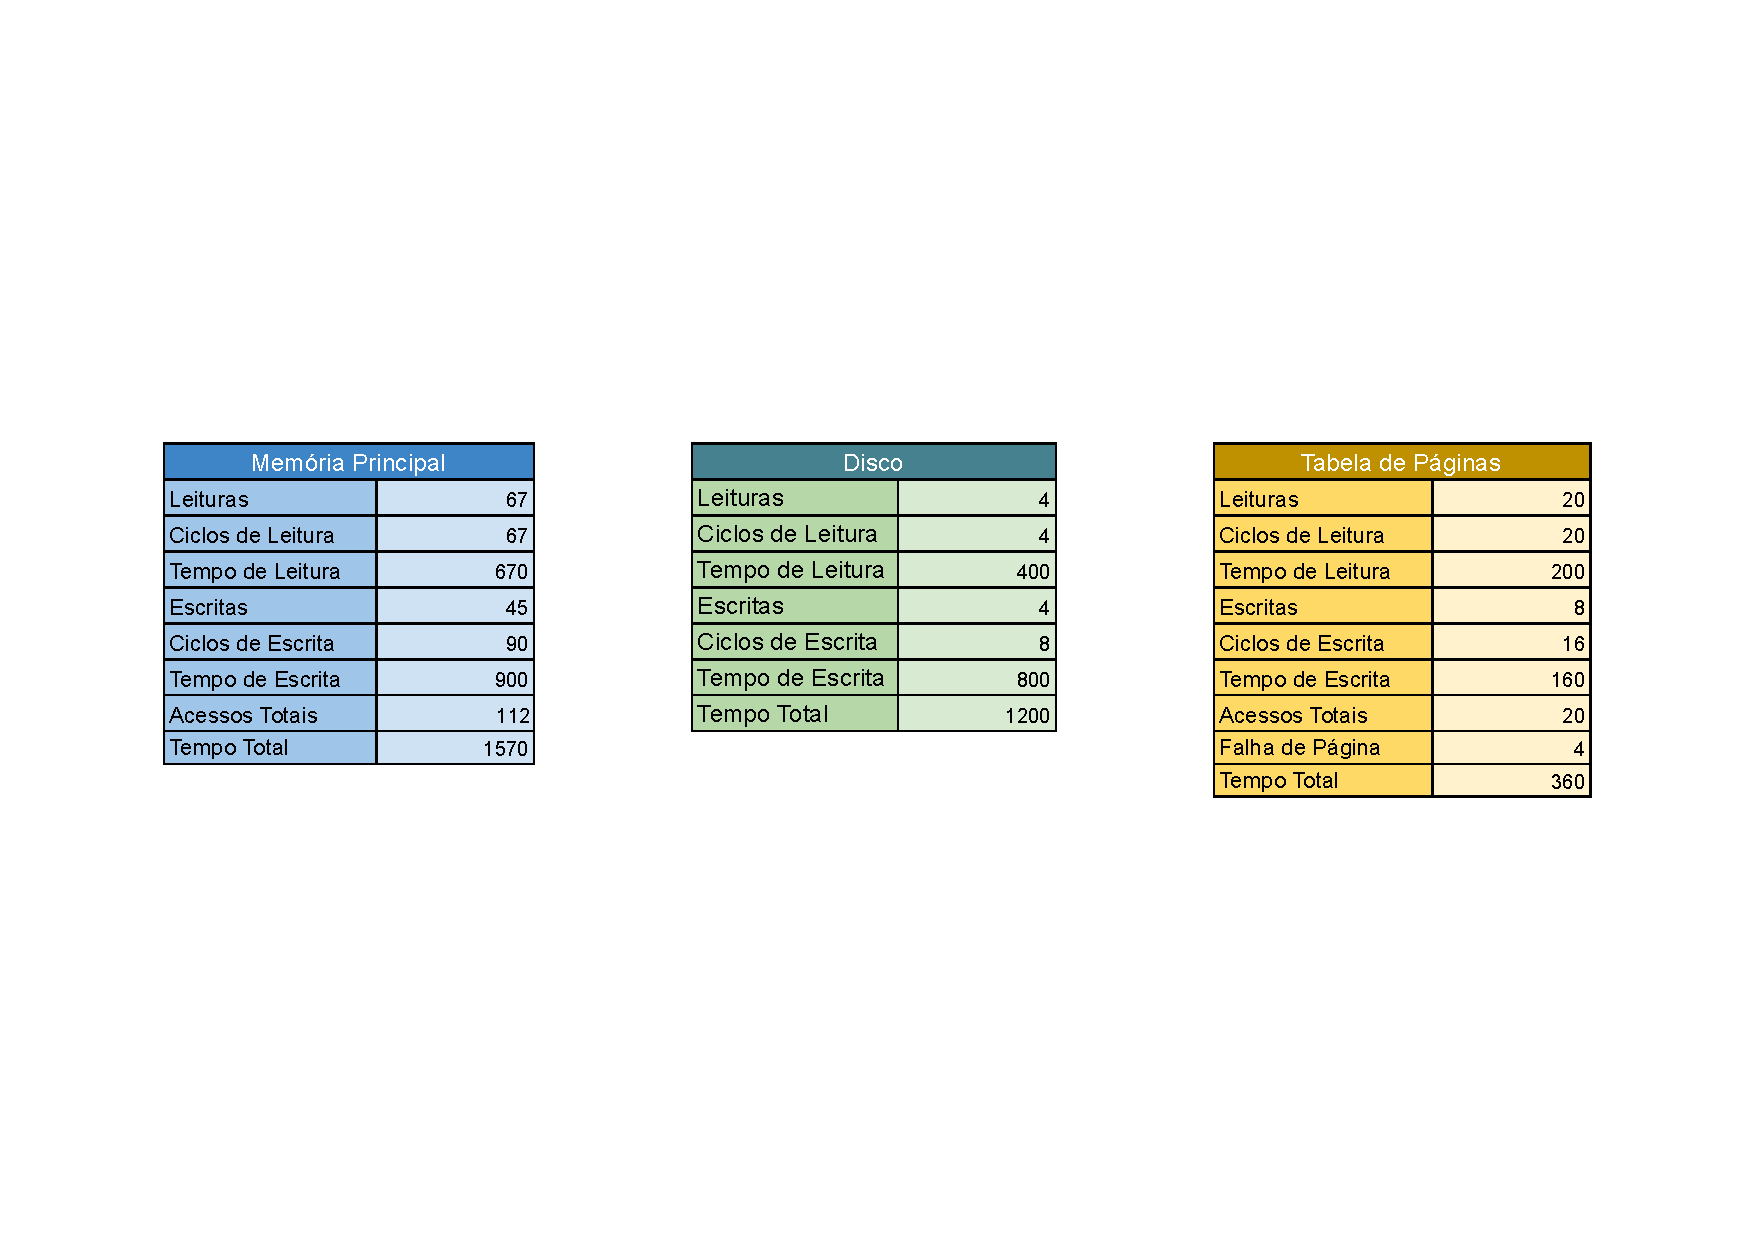
\includegraphics[scale=0.5]{figuras/FIFO-TLB(none).pdf}
  \caption{Tabela com informações da execução do algoritmo FIFO.}
  \label{fig:fifo}
\end{figure}

\subsubsection{LRU}
\label{subsubsec:lru}

A Figura~\ref{fig:lru} mostra as informações sobre a execução do \textit{trace} na arquitetura utilizando o LRU. O tempo total de execução deste \textit{trace} foi de 1660.
É possível observar que o maior tempo gasto desta arquitetura durante as execuções foi na memória principal, em especial nas operações de escrita, que tomaram um total de 51 ciclos e 510 unidades de tempo.

\begin{figure}[H]
  \centering
  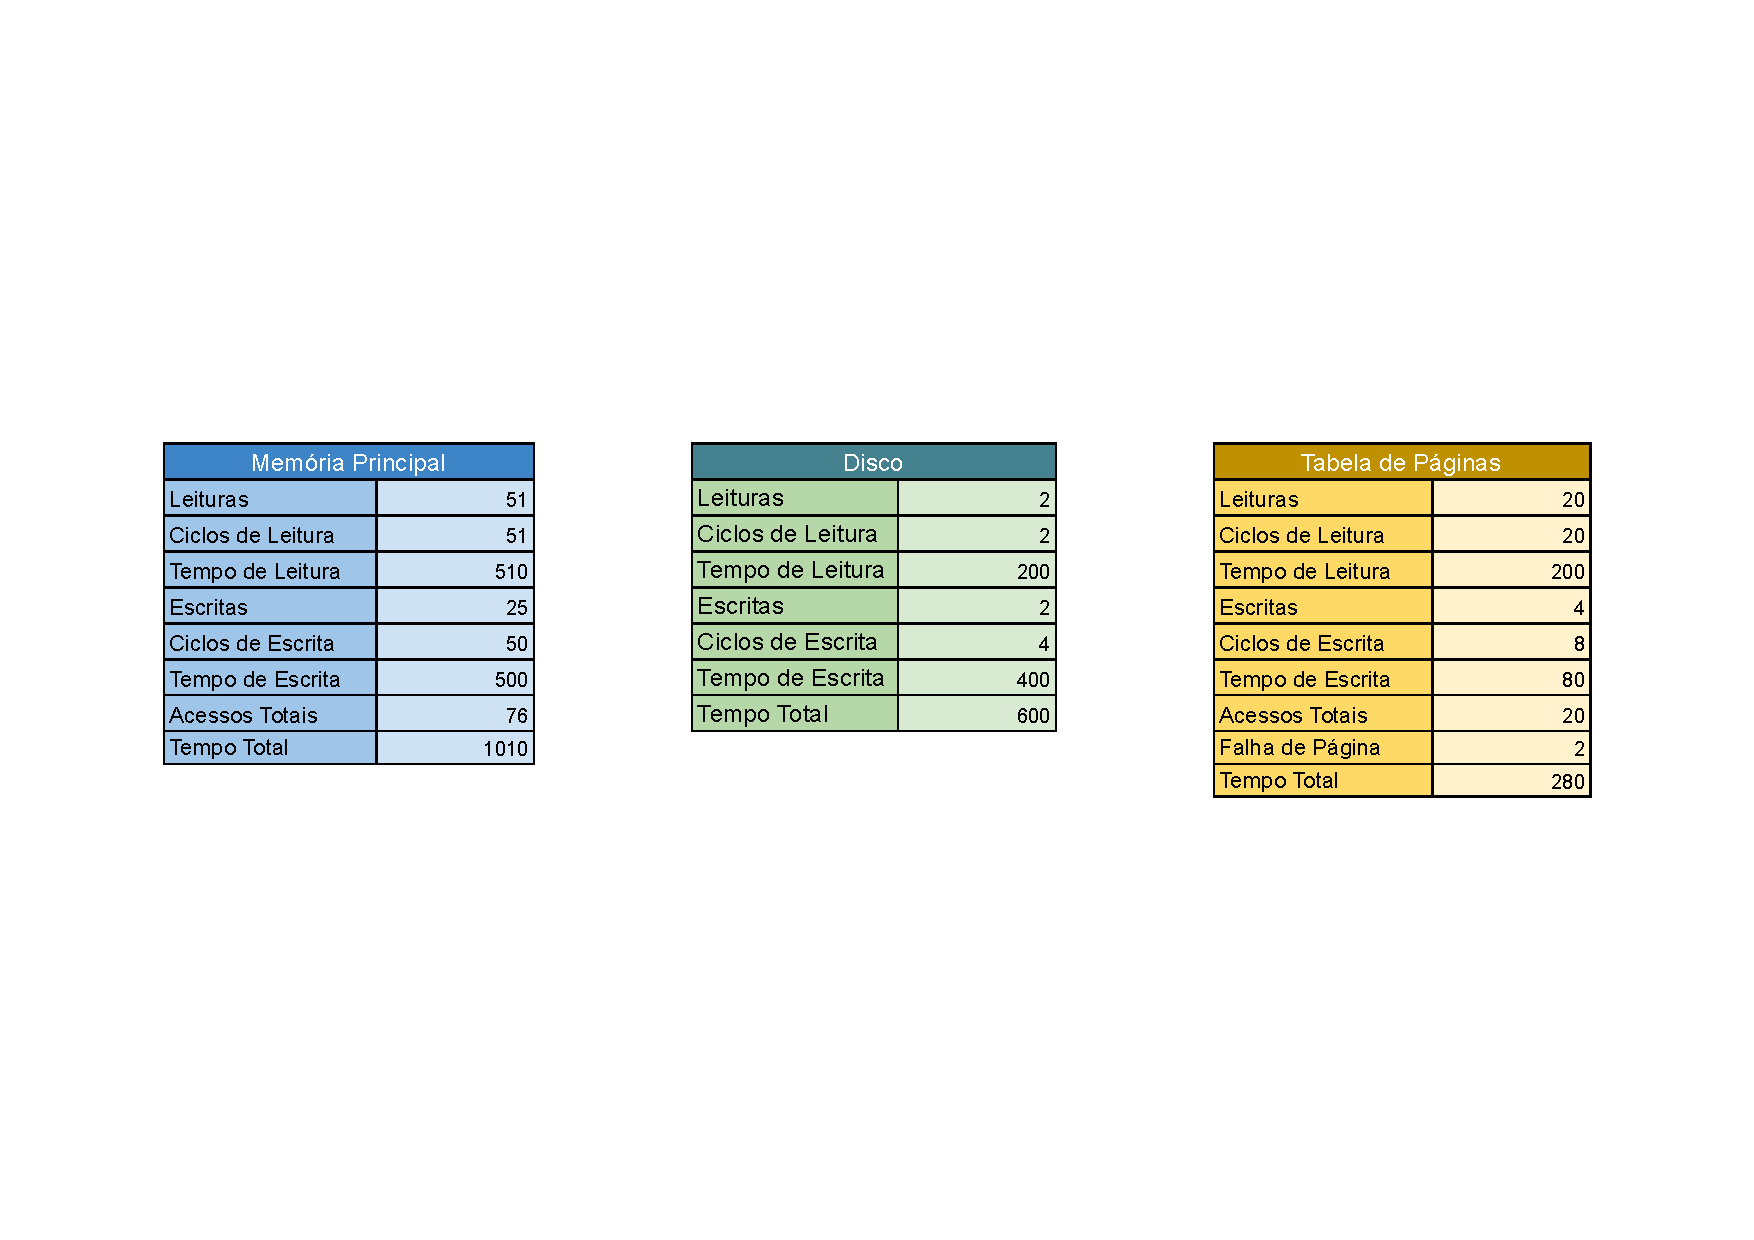
\includegraphics[scale=0.5]{figuras/LRU-TLB(none).pdf}
  \caption{Tabela com informações da execução do algoritmo LRU.}
  \label{fig:lru}
\end{figure}

\section{Conclusões}
\label{sec:conclusoes}
A análise e simulação de diferentes algoritmos de escalonamento de processos permitiram observar de que forma cada abordagem afeta o desempenho e a eficiência do sistema operacional. Cada algoritmo apresenta vantagens e desvantagens específicas, especialmente no que diz respeito a questões como tempo de resposta, utilização da CPU e eficiência. A comparação entre essas abordagens proporcionou uma visão detalhada de seus efeitos no desempenho global, auxiliando na escolha do algoritmo mais adequado conforme as necessidades específicas do sistema e das aplicações em execução.

% ----------------------------------------------------------
% ELEMENTOS PÓS-TEXTUAIS
% ----------------------------------------------------------
\postextual
% ----------------------------------------------------------
% Referências bibliográficas
% ----------------------------------------------------------
\renewcommand{\bibsection}{%
\section{\bibname}
\bibmark
%\ifnobibintoc\else
%\phantomsection
%\addcontentsline{toc}{section}{\bibname}
%\fi
\prebibhook}

\bibliography{abntex2-modelo-references}

\end{document}
